% ==================================================
% Linear Model 
% Author: Lester James V. Miranda
% ==================================================

\documentclass[preview, convert={outfile=\jobname.png,density=300}]{standalone}

\usepackage{tikz}
\usepackage{color}
\usepackage{subfig}
\usepackage{ifthen}
\usepackage{graphicx}
\usepackage{fontawesome}

\renewcommand\familydefault{\sfdefault}

\usetikzlibrary{
    matrix,
    shapes,
    fit,
    arrows,
    positioning,
    calc,
    backgrounds,
    shadows.blur,
    shapes.geometric,
}

\begin{document}
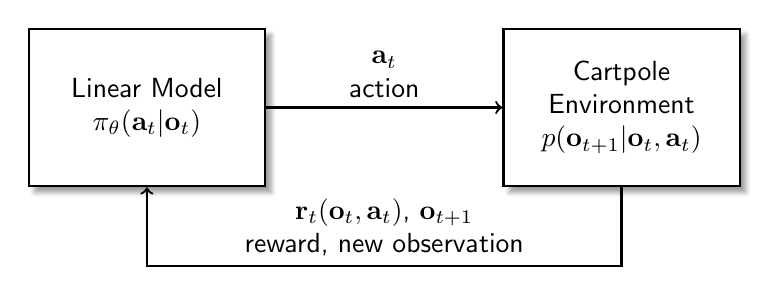
\begin{tikzpicture}[
    node distance = 3cm,
    state/.style={draw, thick, align=center, minimum width=3cm, minimum height=2cm, fill=white, text=black, blur shadow={shadow blur steps=5}},
    ]

\node[state] at (0,0) (linear)
    {Linear Model\\$\pi_{\theta}(\mathbf{a}_{t} \vert
    \mathbf{o}_{t})$};

\node[state] [right=of linear] (cartpole)
    {Cartpole\\Environment\\$p(\mathbf{o}_{t+1} \vert
    \mathbf{o}_{t}, \mathbf{a}_{t})$};

\draw[->, thick] (linear) -- (cartpole) node[midway, above, align=center]
    {$\mathbf{a}_{t}$\\action};

\draw[->, thick] (cartpole.south) |- ++(0,-1cm) -| (linear.south)
    node[pos=0.25, above, align=center] {$\mathbf{r}_{t}(\mathbf{o}_{t},
    \mathbf{a}_{t})$, $\mathbf{o}_{t+1}$\\reward, new observation};


\end{tikzpicture}
\end{document}
